\documentclass{article}

\usepackage[italian]{babel}
\usepackage[margin=2cm, footskip=5mm]{geometry}
% questi package non sono necessari in lualatex; ref https://tex.stackexchange.com/a/413046
% \usepackage[utf8]{inputenc}
% \usepackage[T1]{fontenc}
\usepackage{enumitem}
\usepackage{hyperref}
\usepackage{titlesec}
\usepackage{soulutf8}
\usepackage{contour}
\usepackage{float}
\usepackage{graphicx}
\usepackage{fancyhdr}
\usepackage{longtable}
\usepackage[table]{xcolor}
\usepackage{titling}
\usepackage{lastpage}
\usepackage{ifthen}
\usepackage{calc}
\usepackage{minted}
\usepackage{pgfgantt}
\usepackage{subfiles}

\newlength{\imgwidth}

\newcommand\scalegraphics[1]{%
    \settowidth{\imgwidth}{\includegraphics{#1}}%
    \setlength{\imgwidth}{\minof{\imgwidth}{\textwidth}}%
    \includegraphics[width=\imgwidth]{#1}%
}

% XXX definizione dei percorsi in cui cercare immagini
\graphicspath{ {./}
    {./img/}
}

% esempio di utilizzo: \appendToGraphicspath{./img/} (un comando diverso per ogni path da includere)
% N.B.: ci DEVE essere un forward slash alla fine del path, a indicare che è una cartella.
\makeatletter
\newcommand\appendToGraphicspath[1]{%
  \g@addto@macro\Ginput@path{{#1}}%
}
\makeatother

% setup della sottolineatura
\setuldepth{Flat}
\contourlength{0.8pt}

\newcommand{\uline}[1]{%
  \ul{{\phantom{#1}}}%
  \llap{\contour{white}{#1}}%
}

% setup dei link
\hypersetup{
  colorlinks=true, % set true if you want colored links
  linktoc=all,     % set to all if you want both sections and subsections linked
  linkcolor=black, % choose some color if you want links to stand out
}

% setup di header e footer
\pagestyle{fancy}

\fancyhf{}
\fancyhead[L]{\includegraphics[width=1cm]{logo.png}}
\fancyhead[R]{\thetitle}
\fancyfoot[R]{\thepage\ di~\pageref{LastPage}}

\fancypagestyle{nopage}{%
  \fancyfoot{}%
}

\setlength{\headheight}{1.2cm}

% setup forma \paragraph e \subparagraph
\titleformat{\paragraph}[hang]{\normalfont\normalsize\bfseries}{\theparagraph}{1em}{}
\titleformat{\subparagraph}[hang]{\normalfont\normalsize\bfseries}{\thesubparagraph}{1em}{}

% setup profondità indice di default
\setcounter{secnumdepth}{5}
\setcounter{tocdepth}{5}

% shortcut per i placeholder
\newcommand{\plchold}[1]{\textit{\{#1\}}} % chktex 20

% hook per lo script che genera il glossario
\newcommand{\glossario}[1]{\underline{#1}\textsubscript{g}}

% definizione dei comandi \uso e \stato
\makeatletter
\newcommand{\setUso}[1]{%
  \newcommand{\@uso}{#1}%
}
\newcommand{\uso}{\@uso}

\newcommand{\setStato}[1]{%
  \newcommand{\@stato}{#1}%
}
\newcommand{\stato}{\@stato}

\newcommand{\setVersione}[1]{%
  \newcommand{\@versione}{#1}%
}
\newcommand{\versione}{\@versione}

\newcommand{\setResponsabile}[1]{%
  \newcommand{\@responsabile}{#1}%
}
\newcommand{\responsabile}{\@responsabile}

\newcommand{\setRedattori}[1]{%
  \newcommand{\@redattori}{#1}%
}
\newcommand{\redattori}{\@redattori}

\newcommand{\setVerificatori}[1]{%
  \newcommand{\@verificatori}{#1}%
}
\newcommand{\verificatori}{\@verificatori}

\newcommand{\setDescrizione}[1]{%
  \newcommand{\@descrizione}{#1}%
}
\newcommand{\descrizione}{\@descrizione}

\newcommand{\setModifiche}[1]{%
  \newcommand{\@modifiche}{#1}%
}

\newcommand{\modifiche}{\@modifiche}

\makeatother

% setup delle description
\setlist[description,1]{font=$\bullet$\hspace{1.5mm}, labelwidth=* leftmargin=*,labelindent=12.5mm}
\setlist[description,2]{font=$\bullet$\hspace{1.5mm}, leftmargin=*,labelindent=12.5mm}
\appendToGraphicspath{../../commons/img/}

\title{Verbale esterno --- 02/04/2020}

\setResponsabile{Alberto Cocco}
\setRedattori{Alessandro Rizzo}
\setVerificatori{
  Alberto Cocco
}
\setUso{Esterno}
\setDescrizione{Verbale dell'incontro di GruppOne del 02/04/2020}
\setModifiche{%
\cellcolor{white!80!lightgray!100} & Alberto Cocco & 2020--04--04 & approva documento \\%
\cellcolor{white!80!lightgray!100} & Verificatori & 2020--04--03 & verifica verbale \\%
\multirow{-3}{*}{0.1.2} \cellcolor{white!80!lightgray!100} & Alessandro Rizzo & 2020--04--02 & stendi verbale %
}

\disabilitaVersione{}
\disabilitaElencoFigure{}
\disabilitaElencoTabelle{}

\begin{document}

\thispagestyle{empty}
\pagenumbering{gobble}

\begin{center}

  \includegraphics[width=8.5cm]{\commons/img/logo.png}\\
  {\Large GruppOne - progetto "Stalker"}\\
  \vspace{1.5cm}

  {\Huge \thetitle}
  \vspace{1.5cm}

  \begin{table}[H]
    \centering

    \begin{tabular}{r|l}
      \textbf{Versione}     & \versione              \\
      \textbf{Approvazione} & \responsabile          \\
      \textbf{Redazione}    & \redattori             \\
      \textbf{Verifica}     & \verificatori          \\
      \textbf{Stato}        & \stato                 \\
      \textbf{Uso}          & \uso                   \\
      \textbf{Destinato a}  & Imola Informatica      \\
                            & GruppOne               \\
                            & Prof. Tullio Vardanega \\
                            & Prof. Riccardo Cardin  \\
    \end{tabular}
  \end{table}

  \vspace{3cm}
  \textbf{Descrizione}\\
  \descrizione\\
  \vfill
  \verb|gruppone.swe@gmail.com|
\end{center}

\newpage
\thispagestyle{nopage}

\section*{Registro delle modifiche}
\label{sec:registro_delle_modifiche}

\begin{table}[H]
  \label{tab:registro_delle_modifiche}

  \centering
  \rowcolors{2}{lightgray}{white!80!lightgray!100}

  \begin{longtable}[c]{c c c c l}
    \rowcolor{darkgray!90!}\color{white}{\textbf{Versione}} & \color{white}{\textbf{Data}} & \color{white}{\textbf{Nominativo}} & \color{white}{\textbf{Ruolo}} & \color{white}{\textbf{Descrizione}} \\\endhead
    \modifiche
  \end{longtable}
\end{table}

% section registro_delle_modifiche (end)
\newpage

\thispagestyle{nopage}
\pagenumbering{roman}
\tableofcontents

\newpage

\pagenumbering{arabic}


\section{Informazioni logistiche}%
\label{sec:informazioni_logistiche}

\begin{description}
  \item [Luogo] Hangouts
  \item [Data] 02/04/2020
  \item [Ora] 14:30 \symbol{8594} 15:30
\end{description}

\subsection{Membri del gruppo presenti}%
\label{sub:membri_del_gruppo_presenti}

\begin{enumerate}
  \item Riccardo Agatea
  % \item Tobia Apolloni
  \item Riccardo Cestaro
  \item Alberto Cocco
  \item Luca Ercole
  \item Alberto Gobbo
  \item Alessandro Rizzo
  \item Fabio Scettro
\end{enumerate}

% sub:membri_del_gruppo_presenti (end)

\subsection{Altri partecipanti}%
\label{sub:altri_partecipanti}

\begin{enumerate}
  \item Davide Zanetti (Imola Informatica, proponente del capitolato)
\end{enumerate}

% sub:altri_partecipanti (end)
% sec:informazioni_logistiche (end)

\section{Introduzione}%
\label{sec:introduzione}
L'incontro è avvenuto tramite chiamata Hangouts.
Lo scopo principale era discutere del lavoro del gruppo nelle ultime settimane e confrontarsi sui risultati ottenuti.

\section{Ordine del giorno}%
\label{sec:ordine_del_giorno}

\begin{itemize}
  \item discussione app
  \item salvataggio degli accessi nel server
  \item discussione web-app
  \item protocollo REST
  \item server LDAP
  \item Spring
  \item Reactive Stack
\end{itemize}

\section{Discussione App}%
\label{sec:discussione_app}
Il proponente ha approvato il lavoro svolto finora sull'applicazione mobile e ci ha consigliato un contatto all'interno di Imola Informatica a cui rivolgere domande specifiche sullo sviluppo Android.
% sec:discussione_app (end)

\section{Salvataggio degli accessi nel server}%
\label{sec:salvataggio_accessi_server}
Abbiamo spiegato al proponente l'idea di avere due database separati, uno per i dati utente e uno per lo storico delle posizioni.
Il proponente ha approvato il nostro lavoro e ci consiglia di tenere un report delle posizioni con il campo dati per l'ID utente opzionale per supportare entrambe le modalità di localizzazione.
Abbiamo anche concordato fosse importante prestare attenzione al costo computazionale di effettuare query sugli utenti o sui luoghi e quale sarebbe stata quella più utilizzata al fine di ottimizzarla.
% sec:salvataggio_accessi_server (end)

\section{Discussione web-app}%
\label{sec:discussione_web_app}
Abbiamo mostrato quanto svolto finora al proponente che è sembrato soddisfatto, in particolare dell'utilizzo di un framework che consente di creare una mappa interattiva come era richiesto in via opzionale nel capitolato.
% sec:discussione_web_app (end)

\section{Protocollo REST}%
\label{sec:protocollo_rest}
Abbiamo chiesto al proponente cosa intendesse specificatamente con il termine ``API RESTful'' all'interno del capitolato, in particolare se fosse necessario arrivare al terzo livello di \glossario{REST} e implementare il protocollo \glossario{HATEOAS} nelle chiamate http.
Il proponente ha spiegato che il terzo livello è molto interessante a livello concettuale ma anche molto complesso da implementare a livello di API, ha quindi concluso che sarebbe certamente un valore aggiunto ma che per questo progetto è sufficiente il secondo livello, su cui abbiamo già impostato la nostra API\@.
% sec:protocollo_rest (end)

\section{server LDAP}%
\label{sec:server_ldap}
Abbiamo chiesto una conferma al proponente sulla nostra idea di salvare l'indirizzo http del server \glossario{LDAP} e creare una domanda da inviare all'indirizzo salvato quando un utente desidera autenticarsi ad una organizzazione, il proponente ha confermato le nostre idee.
% sec:server_ldap (end)

\section{Spring}%
\label{sec:spring}
Il proponente in seguito ad una domanda riguardo l'apprendimento del framework \glossario{Spring} ci ha consigliato di non perdere troppo tempo nella documentazione ma di cercare esempi che rappresentino al meglio il nostro caso e nel caso servissero informazioni specifiche di andare sempre prima sul sito StackOverflow.
% sec:spring (end)

\section{Reactive Stack}%
\label{sec:reactive_stack}
Alla richiesta del gruppo di un parere sull'utilizzo di \glossario{Reactive Stack} per lo sviluppo del server il proponente ha consigliato di verificare prima la compatibilità delle scelte tecnologiche dei database con Reactive e di utilizzare il plugin Spring Data Reactive.
% sec:reactive_stack (end)


\newpage
\section{Registro delle decisioni}%
\label{sec:registro_delle_decisioni}

\begin{description}
  \item[20200402-ext-001] Abbiamo deciso di proseguire con il lavoro come da preventivo integrando gli spunti che il proponente ci ha fornito.
\end{description}

\end{document}
